\documentclass{beamer}
%%% PACKAGES
\usepackage[russian]{babel}
\usepackage[utf8]{inputenc}
\usepackage{amsmath}
\usepackage{amssymb}
\usepackage{tikz}
\usepackage{graphics}
\usepackage{color}
\usepackage{algorithmicx}
\usepackage{algpseudocode}
\usepackage[]{algorithm2e}

%%% BEAMER SETTINGS
\setbeamertemplate{navigation symbols}{}
\setbeamertemplate{headline}{}

%%% TIKZ SETTINGS
\usetikzlibrary{fit}

%%% NEW COMMANDS
\def\pitem{\pause \item}

\usetheme{Madrid}

\begin{document}


\title[Оценки задачи Needle]{Верхние и нижние оценки несмещенной вычислительной сложности
оптимизационной задачи Needle}

\author[Виктория Волочай] {Виктория Волочай Олеговна}

\institute[Университет ИТМО]{
{
    \begin{figure}[h]
    
\includegraphics[height=1.5cm]{itmo.png}
    \end{figure}
}

\vspace{1.7em}
Научный руководитель - к.т.н М.В.Буздалов}

\date{СПИСОК, 29.04.2016}

\subject{Theoretical Computer Science}

\begin{frame}
  \titlepage
\end{frame}

 \begin{frame}{План презентации}
  \tableofcontents
 \end{frame}

 \section{Введение}
 
 \subsection{Needle}
 \begin{frame}{Needle}
  \begin{itemize}
   \item Загадана битовая строка z, длина которой известна и равна n. Сама же битовая строка неизвестна.
   \item  Для всех $z \in \{0, 1\}^n \;\;\; $  
    \begin{math} 
    f_{z} : \{0, 1 \}^n \rightarrow \{0,1\}; x \rightarrow  \left\{ \begin{array}{ll}
    1 & \textrm{$x = z$}\\
    0 & \textrm{$x \ne z$}
    \end{array} \right.
    \end{math}

   \item Класс задач $Needle_n$ - это множество задач $Needle_{n, z}$ для всех z.
   \end{itemize} 
 \end{frame}

% 2план презентации
% 3мотивация
% 4black-box-comlexity
% 5Несмещенные операторы
% 6Алгоритм несмещенных с black-box
% 7Needle
% 8Тернарный оператор: пример
% 9Бинарный оператор
% 10Унарный оператор
% 11Дальнейшая работа


 \subsection{Black-box сложность}
 
 \begin{frame}{Black-box complexity}
    Задача представлена оптимизирующему алгоритму в виде черного ящика, к которому можно делать запросы, и он возвращает 1, если запрос совпадает со строкой z, и 0 в противном случае.
    \begin{figure}[h]
    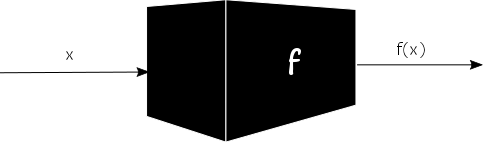
\includegraphics[height=2cm]{blackbox.png}
    \end{figure}
    Black-box дает оценку сложности алгоритма, не имеющего полных знаний о решаемой задаче.   
 \end{frame}
 
 
  \begin{frame}{Black-box сложность: верхние и нижние оценки}
  \begin{itemize}
   \item Верхняя оценка
        \begin{itemize}
            \item Создание алгоритма для решения задачи и оценка  времени работы
            \item Алгоритм может быть не эволюционным
        \end{itemize}
    \item Нижняя оценка
        \begin{itemize}
            \item Доказательство того, что сложность алгоритма не может быть меньше какой-то величины.
            \item Гораздо сложнее находятся, чем верхние границы.
        \end{itemize}
    \end{itemize}
 \end{frame}

 
%\begin{frame}{Black-box complexity} 
%Black-box complexity описывает ``сложность'' задач при решении алгоритмами, не имеющими доступа к определению решаемой задачи 
% Для многих задач наилучший black-box алгоритм работает намного быстрее, чем существующие эволюционные подходы 
% Недавно был предложен способ модификации эволюционного алгоритма, основанный на идеях из black-box complexity, увеличивающий эффективность использования алгоритмом получаемой информации 


 \begin{frame}{Вычислительная сложность Needle}
  \begin{itemize}
   \item Вычислительная сложность $Needle_n$ по отношению ко всем возможным алгоритмам равна $(2^n + 1) / 2$.
   \item Такое же время работы у алгоритма, который генерирует
случайную перестановку чисел от 0 до $(2^n - 1)$
   \item Верхняя и нижняя оценка совпадают.
  \end{itemize}
 \end{frame} 


  \begin{frame}{Мотивация}
  \begin{itemize}
   \item Needle является одной из сложных задач, так как за запрос алгоритм не получает никакой информации.
   \item Сложность работы алгоритма равна $(2^n + 1) / 2$. Необходимо получить более точные оценки.
   \item Возможно, идеи решения задачи Needle помогут решить плато. 
   \item Алгоритм (1+1) оптимизирует гораздо медленнее. Необходимо понять, как устроены эти алгоритмы и какие несмещенные операторы к ним уместно применять.
   
  \end{itemize}
 \end{frame}


 \section{Несмещенные алгоритмы арности k}
 
 \begin{frame}{Несмещенные алгоритмы арности k}
  \begin{itemize}
   \item Запрос $Q_1$ - запрос, сгенерированный случайным образом.
   \item Запрос $Q_{i+1}$ - реализация случайной величины, такой что:
        \begin{itemize}
            
            \item  Для любой z $$ p(Q_{i+1} | Q_1, ... Q_i, A_1, ... A_i) = p(Q_{i+1} \oplus z | Q_1 \oplus z, ..., Q_i \oplus z, A_1, ..., A_i)$$  
            
            \item Для любой перестановки perm() 
            $  p(Q_{i+1} | Q_1, ..., Q_i, A_1, ..., A_i) = p(perm(Q_{i+1}) |perm(Q_1), ..., perm(Q_i), A_1, ... A_i) $ 
            
        \end{itemize}

 \item Алгоритм арности k: случайная величина, генерирующая $Q_{i+1}$ рандомизировано выбирает не более k различных индексов $H_j$ из $[1; i]$ и генерирует $Q_{i+1}$ используя только $Q_{H_1}, ..., Q_{H_K}, A_{H_1}, ... A_{H_K}$
  \end{itemize}
 \end{frame}
 
 \begin{frame}{Black-box алгоритм для несмещенных операторов} 
    \begin{algorithm}[H]
    \textrm{Выбрать $x^0$ равномерно случайно из $\{0,1\}^n$ и запросить $f(x^0)$ } \\
    \For{t = 1,2,3... \textrm{до окончания работы} }{
    \textrm{В зависимости от $f(x^0),...,f(x^{t-1})$ выбрать несмещенный оператор порядка $k p^t$ и $k$ запрошенных ранее точек $x^i,...,x^{ik}$ } \\
    \textrm{Выбрать $x^t$ из $p^{t} (x^{i_1},...,x^{i_k})$ и запросить $f(x^t)$}
    }
    \EndFor
    \end{algorithm}
 \end{frame}

 \subsection{Тернарный оператор}
 \begin{frame}{Алгоритм для k = 3}
    \begin{enumerate}
        \item flip one bit
        \item flip'(a,b) такой что:
        \begin{itemize}
            \item выбрать i совпадающих бит в $а$ и $b$ 
            \item flip one bit
        \end{itemize}
        
        \item $ xor3(a,b,c):  a \oplus b \oplus c $
    \end{enumerate}
 \end{frame}



 \begin{frame}{Алгоритм для k = 3}
  \begin{itemize}
  \item {
        \begin{minipage}{0.4\textwidth}
            \begin{math} q_0 \leftarrow & \textrm{random}
            \end{math}
        \end{minipage}
        \hfill
        \begin{minipage}{0.4\textwidth}
        [0000...0000]
        \end{minipage}
    \pause 
  }
  \item {   
        \begin{minipage}{0.4\textwidth}
        \begin{math}  s_1 \leftarrow & \textrm{flip one bit}
        \end{math}
        \end{minipage}
        \hfill
        \begin{minipage}{0.4\textwidth}
        [0000...0001]
        \end{minipage}
  }
  % You can also specify when the content should appear
  % by using <n->:
  \item<3-> {
        \begin{minipage}{0.4\textwidth}
        \begin{math}  s_2 \leftarrow & \textrm{flip'$(q_0, s1)$}
        \end{math}
        \end{minipage}
        \hfill
        \begin{minipage}{0.4\textwidth}
        [0000...0010]
        \end{minipage}

  }
  \item<4-> {
        \begin{minipage}{0.4\textwidth}
        \begin{math} t_2 \leftarrow & \textrm{xor $(q_0, s1, s2)$}
        \end{math}
        \end{minipage}
        \hfill
        \begin{minipage}{0.4\textwidth}
        [0000...0011]
        \end{minipage}
  }
  % or you can use the \uncover command to reveal general
  % content (not just \items):
  \item<5-> {
        \begin{minipage}{0.4\textwidth}
        \begin{math} s_3 \leftarrow & \textrm{flip' $(q_0, s2)$}
        \end{math}
        \end{minipage}
        \hfill
        \begin{minipage}{0.4\textwidth}
        [0000...0100]
        \end{minipage}

  }
  \item <6->{...}
  \item <7->{
        \begin{minipage}{0.4\textwidth}
        \begin{math} s_n = 
        \end{math}
        \end{minipage}
        \hfill
        \begin{minipage}{0.4\textwidth}
        [1000...0000]
        \end{minipage} \\
  Оценка работы алгоритма равна $(2^n + 1) / 2$ \\
  При k = 3 будет достигнут оптимум.
  }
  \end{itemize}
\end{frame}

 
 \subsection{Бинарный оператор}
 \begin{frame}{Оценка для k = 2}
 \begin{math}
    x_0 \leftarrow & \textrm{random} \\
    x_1 \leftarrow & \textrm{$x_0$ flip m bit} \\
 \end{math}
 Пространство поиска:
    \begin{figure}[h]
    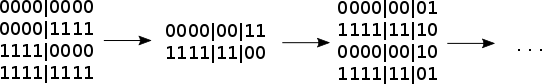
\includegraphics[height=1.5cm]{binary.png}
    \end{figure}
    
 Оценка работы:  $2^n - 2n + const$
 \end{frame}
 
 
 \subsection{Унарный оператор}
 \begin{frame}{Оценка для k = 1}
    \begin{itemize}
    \item 
    \begin{math} 
        x_0 \leftarrow & \textrm{random} \\
        \textrm{Разобьем пространство поиска на классы} \\
        d_1 : n \\
        d_2 : \binom{n}{2} \\
        . \\
        . \\
        
        d_{n-1} : \binom{n}{n-1} = n \\
        d_{n} : 1 \\    
    \end{math}
    \item E(d, i) - матожидание числа различных запросов на  расстояние d, если на этом расстоянии сделано i запросов.
    \item E(d, i) - E(d, i - 1)
    \item Оценка работы алгоритма $2^n - n + const$
    \end{itemize}
 \end{frame}

\section{Заключение}

\begin{frame}{Дальнейшая работа}
  \begin{itemize}
  \item
    Получение более точных оценок на унарный оператор.
  \item
    Найти подходящую функцию для максимизации количества особей при $k=2$ 
  \end{itemize}
\end{frame}

 \begin{frame}
    \center Cпасибо!
 \end{frame}
 
 \end{document}